%  !TeX  root  =  user_guide.tex
\chapter{Aperçu des fonctionnalités} \label{feature_glance}

Après une première prise en main dans le chapitre \ref{label_getstarted}, nous allons maintenant vous donner un aperçu plus détaillé des fonctionnalités de \qg. La plupart seront décrites plus précisément encore dans les chapitres qui leur sont dédiés dans la suite du manuel.

\section{Démarrer et arrêter \qg} \label{label_starting}

Dans le chapitre \ref{samplesession}, vous avez appris comment démarrer \qg. Nous allons répéter cette étape ici et vous verrez que \qg propose des options supplémentaires via la ligne de commande.

\begin{itemize}[label=--]
\item \nix{en présumant que \qg est installé dans le PATH (chemin par défaut), vous pouvez le démarrez en tapant : \usertext{qgis}  dans une ligne de commande ou en cliquant sur l'icône de raccourci sur le bureau dans le menu des applications.} 
\item \win{démarrez \qg en utilisant le menu Démarrer, l'icône de raccourci présent sur le bureau ou encore, en cliquant sur un fichier de projet \qg}
\item \osx{double-cliquez sur l'icône de votre répertoire Applications. Si vous avez besoin d'exécuter \qg dans une console, lancez avec \mbox{/chemin-vers-exécutable/Contents/MacOS/qgis}.}
\end{itemize} 

Pour arrêter \qg, cliquez sur le menu \{\nix{} \win{Fichier} \osx{Qgis} \} > Quitter, ou utilisez le raccourci clavier \keystroke{Ctrl+Q} (osx{\keystroke{cmd+Q}}).

\subsection{Options de ligne de commande} \index{options de ligne de commande}
\label{label_commandline}

\nix \qg supporte un certain nombre d'options lorsque démarré en passant par la ligne de commande. Pour obtenir une liste de ces options, entrez dans votre console \usertext{qgis ---help}. Le message habituel qui en résulte est :

\small
\begin{verbatim}
QGIS --help
Quantum GIS - 1.5.0-Thetys 'Thetys' (exported)
Quantum GIS (QGIS) est un visualisateur de données spatiales, raster ou vecteur.
Usage: QGIS [options] [FILES]
  options:
		[--snapshot filename]           emit snapshot of loaded datasets to given file
		[--width width]                 width of snapshot to emit
		[--height height]               height of snapshot to emit
		[--lang language]               use language for interface text
		[--project projectfile]         load the given \qg project
		[--extent xmin,ymin,xmax,ymax]  set initial map extent
		[--nologo]                      hide splash screen
		[--noplugins]                   don't restore plugins on startup
		[--optionspath path]            use the given QSettings path
		[--configpath path]             use the given path for all user configuration
		[--help]                        this text

  FILES:
    Files specified on the command line can include rasters,
    vectors, and QGIS project files (.qgs):
     1. Rasters - Supported formats include GeoTiff, DEM
        and others supported by GDAL
     2. Vectors - Supported formats include ESRI Shapefiles
        and others supported by OGR and PostgreSQL layers using
        the PostGIS extension
\end{verbatim}
\normalsize

\begin{Tip} \caption{\textsc{Exemple utilisant des options de ligne de commande}}
Vous pouvez démarrer \qg en spécifiant un ou plusieurs fichiers de données. Par exemple, si vous êtes placé dans le répertoire qgis\_sample\_data vous pouvez démarrer \qg avec une couche vectorielle et un fichier raster dès le démarrage avec la commande suivante : 
\usertext{qgis ./raster/landcover.img ./gml/lakes.gml}
\end{Tip}

\minisec{Option \usertext{---snapshot}}
Cette option permet de créer une capture d'écran de l'affichage courant au format PNG. C'est pratique quand vous avez une longue série de projets et que vous voulez générer un aperçu de vos données. L'image ainsi créée fait 800x600 pixels, un nom de fichier peut être ajouté après \usertext{---snapshot}. Cette commande peut être adaptée en utilisant les arguments \usertext{---width} pour la largeur et \usertext{---height} pour la hauteur.

\minisec{Option \usertext{---lang}}
\qg se base sur votre environnement linguistique par défaut pour définir la langue de l'interface. Si vous voulez en changer, vous devez le spécifier en saisissant un code. 
Par exemple, \usertext{---lang=it} provoquera l'utilisation de la version italienne. Une liste des langues intégrées est visible à \url{http://wiki.qgis.org/qgiswiki/TranslatorsCorner}

\minisec{Option \usertext{---project}}
Démarrer \qg avec un projet existant est possible, il suffit d'ajouter l'option \usertext{---project} suivie du nom de votre projet et \qg se lancera avec toutes les couches définies dans ce fichier.

\minisec{Option \usertext{---extent}}
Pour démarrer avec une étendue cartographique spécifique, utilisez cette option. Vous devez ajouter les limites de votre étendue dans l'ordre suivant en les séparant par une virgule :
\begin{verbatim}
--extent xmin,ymin,xmax,ymax
\end{verbatim}

\minisec{Option \usertext{---nologo}}
Cette commande dissimule l'écran de démarrage qui apparaît lors du lancement de \qg.

\minisec{Option \usertext{---noplugins}}
Si vous avez un problème de démarrage lié à une extension, cette option permet de lancer \qg sans les charger (elles seront toujours accessible dans le gestionnaire d'extension).

\minisec{Option \usertext{---optionspath}}
Vous pouvez avoir plusieurs configurations et décider laquelle utiliser en utilisant cette option au démarrage. Lisez la section \ref{subsec:gui_options} pour connaître l'emplacement où votre système d'exploitation entrepose les fichiers de préférences. Il n'y pas pour l'instant de possibilité de spécifier dans quel fichier écrire ces préférences, vous devrez donc faire une copie du fichier original.

\minisec{Option \usertext{---configpath}}
Cette option est similaire à la précédente, mais va plus loin en changeant le chemin par défaut de la configuration utilisateur et foblige QSettings à utiliser ce nouveau répertoire. Cela permet de transporter QGIS sur une clé USB avec tous les paramètres et extensions.

\section{Interface de \qg} \index{fenêtre principale}
\label{label_qgismainwindow}

Quand \qg démarre, l'interface se présente à vous sous la forme affichée Figure : \ref{fig:startup}, page \pageref{fig:startup} (les nombres de 1 à 6 se réfèrent aux six zones majeures de l'interface) :

\begin{figure}[ht]
   \centering
   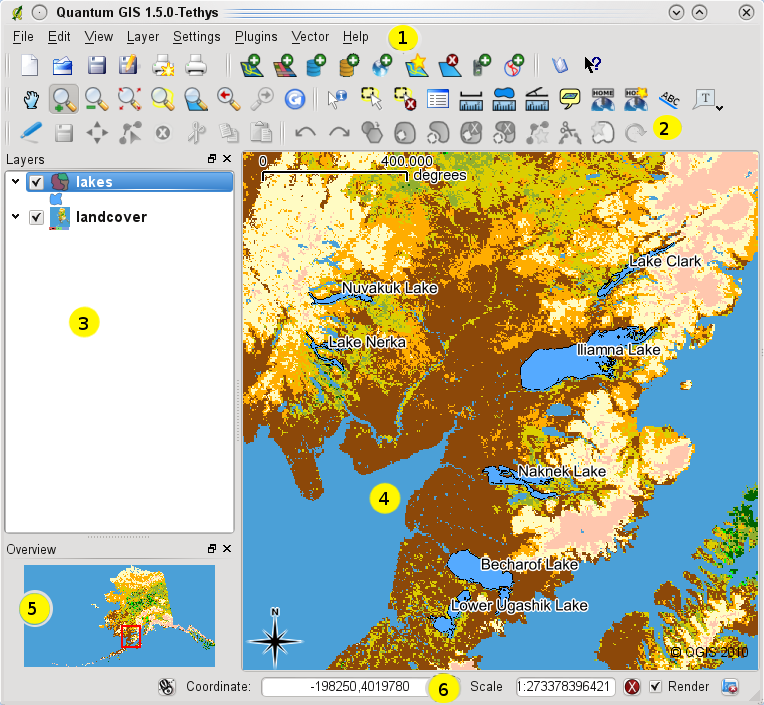
\includegraphics[clip=true, width=12cm]{startup}
   \caption{Interface de \qg avec les données d'essai de l'Alaska \nixcaption. Les numéros cerclés de jaune renvoient aux zones définies dans le texte.} \label{fig:startup}
\end{figure}

\begin{figure}[ht]
   \centering
   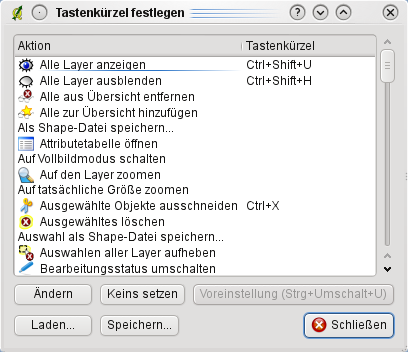
\includegraphics[clip=true, width=8cm]{shortcuts}
   \caption{Fenêtre de configuration des raccourcis \nixcaption (KDE)} \label{fig:shortcuts}
\end{figure}

\textbf{Note:} Les décorations de fenêtre peuvent vous apparaître différemment en fonction de votre système d'exploitation et de votre gestionnaire de fenêtres. \\

L'interface est divisée en 6 zones distinctes :
\begin{center}
\begin{tabular}{p{5cm} p{5cm}}
1. Barre de Menu &4. Affichage de la carte\\
2. Barre d'Outils &5. Aperçu de la carte  \\
3. Légende de la carte &6. Barre de statut \\  
\end{tabular}
\end{center}

Ces 6 composants sont décrits dans les sections suivantes.

\subsection{Barre de Menu} \label{label_menubar}
\index{menus}

La barre de menu fournit un accès aux différentes fonctionnalités de \qg par le biais de menus hiérarchiques. Les entrées du menu de niveau supérieur et un résumé de certaines options sont listés ci-dessous, avec les icônes des outils correspondants dans la barre d'outils et leurs raccourcis clavier \footnote{Les raccourcis clavier peuvent maintenant être configurés manuellement (les raccourcis présentés dans cette section sont ceux par défaut) en utilisant l'outil Configurer les Raccourcis dans le menu Préférences. Les utilisateurs de \osx{} doivent substituer \keystroke{cmd} à \keystroke{Ctrl}.}. L'emplacement de ces entrées varie sensiblement suivant le gestionnaire de fenêtre, donc suivant le système d'exploitation. Bien que les options de menu aient des outils qui leur correspondent et vice-versa, les menus ne sont pas organisés comme les barres d'outils. La barre contenant l'outil est affichée à la suite de chaque option de menu. Pour plus d'informations sur les outils et les barres d'outils, veuillez lire la section \ref{label_barre d'outils}.

{\setlength{\extrarowheight}{10pt}
\small
\begin{longtable}{p{6cm} p{2cm} p{2.5cm} p{2.5cm}}
Option du menu&Raccourci&Référence&Barre d'outils\\
\endfirsthead
Option du menu&Raccourci&Référence&Barre d'outils\\
\endhead
\multicolumn{4}{r}{Fichier} \\
\dropmenuopttwo{mActionFileNew}{Nouveau Projet}&\keystroke{Ctrl+N}&voir Section \ref{sec:projects}&\dropmenucheck{Fichier} \\
\dropmenuopttwo{mActionFileOpen}{Ouvrir un projet...}&\keystroke{Ctrl+O}&voir Section \ref{sec:projects}&\dropmenucheck{Fichier} \\
\dropmenuopt{Ouvrir un projet récent}&&voir Section \ref{sec:projects}&\\
\dropmenuopttwo{mActionFileSave}{Sauvegarder le projet}&\keystroke{Ctrl+S}&voir Section \ref{sec:projects}&\dropmenucheck{Fichier} \\
\dropmenuopttwo{mActionFileSaveAs}{Sauvegarder le projet sous...}&\keystroke{Ctrl+Shift+S}&voir Section \ref{sec:projects}&\dropmenucheck{Fichier} \\
\dropmenuopttwo{mActionSaveMapAsImage}{Sauvegarder comme image...}&&voir Section \ref{sec:output}&\\
\dropmenuopttwo{mActionNewComposer}{Nouveau composeur d'impression}&\keystroke{Ctrl+P}&voir Section \ref{label_printcomposer}&\dropmenucheck{Fichier} \\
\dropmenuopttwo{mActionComposerManager}{Gestionnaire de composeur...}&&voir Section \ref{label_printcomposer}&\dropmenucheck{Fichier} \\
\dropmenuopt{Composeurs d'impression}&&voir Section \ref{label_printcomposer}&\\
\dropmenuopttwo{mActionFileExit}{Quitter}&\keystroke{Ctrl+Q}&&\\
&&&\\
\multicolumn{4}{r}{Éditer} \\
\dropmenuopttwo{mActionUndo}{Annuler}&\keystroke{Ctrl+Z}&voir Section \ref{sec:edit_existing_layer}&\dropmenucheck{Numérisation avancée} \\
\dropmenuopttwo{mActionRedo}{Refaire}&\keystroke{Ctrl+Shift+Z}&voir Section \ref{sec:edit_existing_layer}&\dropmenucheck{Numérisation avancée} \\
\dropmenuopttwo{mActionEditCut}{Couper Entités}&\keystroke{Ctrl+X}&voir Section \ref{sec:edit_existing_layer}&\dropmenucheck{Numérisation} \\
\dropmenuopttwo{mActionEditCopy}{Copier Entités}&\keystroke{Ctrl+C}&voir Section \ref{sec:edit_existing_layer} &\dropmenucheck{Numérisation} \\
\dropmenuopttwo{mActionEditPaste}{Coller Entités}&\keystroke{Ctrl+V}&voir Section \ref{sec:edit_existing_layer}&\dropmenucheck{Numérisation} \\
\dropmenuopttwo{mActionMoveFeature}{Déplacer l'entité}&&voir Section \ref{sec:edit_existing_layer}&\dropmenucheck{Numérisation} \\
\dropmenuopttwo{mActionDeleteSelected}{Supprimer les entités sélectionnées}&&voir Section \ref{sec:edit_existing_layer}&\dropmenucheck{Numérisation} \\
\dropmenuopttwo{mActionSimplify}{Simplifier l'entité}&&voir Section \ref{sec:advanced_edit}&\dropmenucheck{Numérisation avancée} \\
\dropmenuopttwo{mActionAddRing}{Ajouter un anneau}&&voir Section \ref{sec:advanced_edit}&\dropmenucheck{Numérisation avancée} \\
\dropmenuopttwo{mActionAddIsland}{Ajouter une partie}&&voir Section \ref{sec:advanced_edit}&\dropmenucheck{Numérisation avancée} \\
\dropmenuopttwo{mActionDeleteRing}{Effacer un anneau}&&voir Section \ref{sec:advanced_edit}&\dropmenucheck{Numérisation avancée} \\
\dropmenuopttwo{mActionDeletePart}{Effacer une partie}&&voir Section \ref{sec:advanced_edit}&\dropmenucheck{Numérisation avancée} \\
\dropmenuopttwo{mActionReshape}{Remodeler mes entités}&&voir Section \ref{sec:advanced_edit}&\dropmenucheck{Numérisation avancée} \\
\dropmenuopttwo{mActionSplitFeatures}{Séparer les entités}&&voir Section \ref{sec:advanced_edit}&\dropmenucheck{Numérisation avancée} \\
\dropmenuopttwo{mActionMergeFeatures}{Fusionner les entités sélectionnées}&&voir Section \ref{sec:advanced_edit}&\dropmenucheck{Numérisation avancée} \\
\dropmenuopttwo{mActionNodeTool}{Outil de n\oe{}ud}&&voir Section \ref{sec:advanced_edit}&\dropmenucheck{Numérisation avancée} \\
\dropmenuopttwo{mActionRotatePointSymbols}{Rotation des symboles de points}&&voir Section \ref{sec:advanced_edit}&\dropmenucheck{Numérisation avancée} \\
&&&\\
\multicolumn{4}{r}{Après activation du mode édition \toolbtntwo{mActionToggleEditing}{Basculer en mode édition}}\footnote{Activable depuis l'entrée du menu \mainmenuopt{Couche} ou du menu contextuel de la couche, il fait apparaître une icône de création d'entité dans le menu \mainmenuopt{Éditer} selon le type d'entité éditée.} \\
\dropmenuopttwo{mActionCapturePoint}{Créer un point}&\keystroke{.}&voir Section \ref{sec:edit_existing_layer}&\dropmenucheck{Numérisation} \\
\dropmenuopttwo{mActionCaptureLine}{Créer une Ligne}&\keystroke{/}&voir Section \ref{sec:edit_existing_layer}&\dropmenucheck{Numérisation} \\
\dropmenuopttwo{mActionCapturePolygon}{Créer un Polygone}&\keystroke{Ctrl+/}&voir Section \ref{sec:edit_existing_layer}&\dropmenucheck{Numérisation} \\
&&&\\
\multicolumn{4}{r}{Vue} \\
\dropmenuopttwo{mActionPan}{Se déplacer dans la carte}&&&\dropmenucheck{Navigation} \\
\dropmenuopttwo{mActionZoomIn}{Zoom +}&\keystroke{Ctrl++}&&\dropmenucheck{Navigation} \\
\dropmenuopttwo{mActionZoomOut}{Zoom -}&\keystroke{Ctrl+-}&&\dropmenucheck{Navigation} \\
\dropmenuopttwo{mActionSelect}{Sélection d'entités}&&&\dropmenucheck{Attributs} \\
\dropmenuopttwo{mActionDeselectAll}{Désélectionner toutes les entités}&&&\dropmenucheck{Attributs} \\
\dropmenuopttwo{mActionIdentify}{Identifier les entités}&\keystroke{Ctrl+Shift+I}&&\dropmenucheck{Attributs} \\
\dropmenuopttwo{mActionMeasure}{Mesurer une longueur}&\keystroke{Ctrl+Shift+M}&&\dropmenucheck{Attributs} \\
\dropmenuopttwo{mActionMeasureArea}{Mesurer une aire}&\keystroke{Ctrl+Shift+J}&&\dropmenucheck{Attributs} \\
\dropmenuopttwo{mActionMeasureAngle}{Mesurer un angle}&&&\dropmenucheck{Attributs} \\
\dropmenuopttwo{mActionOpenTable}{Zoom sur l'étendue}&\keystroke{Ctrl+Shift+F}&&\dropmenucheck{Navigateur de carte} \\
\dropmenuopttwo{mActionZoomToLayer}{Zoom sur la couche}&&&\dropmenucheck{Navigateur de carte} \\
\dropmenuopttwo{mActionZoomToSelected}{Zoom sur la sélection}&&&\dropmenucheck{Navigateur de carte} \\
\dropmenuopttwo{mActionZoomLast}{Zoom précédent}&&&\dropmenucheck{Navigateur de carte} \\
\dropmenuopttwo{mActionZoomNext}{Zoom suivant}&&&\dropmenucheck{Navigateur de carte} \\
\dropmenuopt{Zoom à la taille réelle}&&&\\
\dropmenuopttwo{mActionMapTips}{Infobulles}&&&\dropmenucheck{Attributs} \\
\dropmenuopttwo{mActionNewBookmark}{Nouveau signet...}&\keystroke{Ctrl+B}&voir Section \ref{sec:bookmarks} &\dropmenucheck{Attributs} \\
\dropmenuopttwo{mActionShowBookmarks}{Montrer les signets}&\keystroke{Ctrl+Shift+B}&voir Section \ref{sec:bookmarks}&\dropmenucheck{Attributs} \\
\dropmenuopttwo{mActionDraw}{Rafraîchir}&\keystroke{Ctrl+R}&&\dropmenucheck{Navigation} \\
\mainmenuopt{Barre d'échelle des tuiles}&&voir Section \ref{sec:tilesets}&\dropmenucheck{Tile scale} \\
\mainmenuopt{Suivi GPS en direct}&&voir Section \ref{sec:gpstracking}&\dropmenucheck{GPS Information} \\
&&&\\
\multicolumn{4}{r}{Couche} \\
\dropmenuopt{Nouveau}&&&\\
\dropmenuopttwo{mActionAddNonDbLayer}{Ajouter une couche vecteur...}&\keystroke{Ctrl+Shift+V}&voir Section \ref{label_workingvector}&\dropmenucheck{Fichier} \\
\mainmenuopt{Calculatrice raster}&&voir Section \ref{sec:raster_calc} \\
\dropmenuopttwo{mActionAddRasterLayer}{Ajouter une couche raster...}&\keystroke{Ctrl+Shift+R}&voir Section \ref{label_raster}&\dropmenucheck{Fichier} \\
\dropmenuopttwo{mActionAddLayer}{Ajouter une couche PostGIS...}&\keystroke{Ctrl+Shift+D}&voir Section \ref{label_postgis}&\dropmenucheck{Fichier} \\
\dropmenuopttwo{mActionAddSpatiaLiteLayer}{Ajouter une couche Spatialite...}&\keystroke{Ctrl+Shift+L}&voir Section \ref{label_spatialite}&\dropmenucheck{Fichier} \\
\dropmenuopttwo{mActionAddWmsLayer}{Ajouter une couche WMS...}&\keystroke{W}&voir Section \ref{sec:ogc-wms}&\dropmenucheck{Fichier} \\
\dropmenuopttwo{mActionOpenTable}{Ouvrir la table d'attributs}&&&\dropmenucheck{Attributs} \\
\dropmenuopttwo{mActionFileSave}{Sauvegarder les modifications}&&&\dropmenucheck{Numérisation} \\
\dropmenuopttwo{mActionToggleEditing}{Basculer en mode édition}&&&\dropmenucheck{Numérisation} \\
\mainmenuopt{Sauvegarder sous...}&&&\\
\mainmenuopt{Enregistrer la sélection en tant que fichier vectoriel}&&&\\
\dropmenuopttwo{mActionRemoveLayer}{Supprimer la couche}&\keystroke{Ctrl+D}&&\dropmenucheck{\scriptsize Gestion des couches} \\
\mainmenuopt{Propriétés...}&&&\\
\mainmenuopt{Requête...}&&&\\
\dropmenuopttwo{mActionInOverview}{Ajouter dans l'aperçu}&\keystroke{Ctrl+Shift+O}&&\dropmenucheck{\scriptsize Gestion des couches} \\
\dropmenuopttwo{mActionAddAllToOverview}{Ajouter tout dans l'aperçu}&&&\\
\dropmenuopttwo{mActionRemoveAllFromOverview}{Enlever tout de l'aperçu}&&&\\
\dropmenuopttwo{mActionHideAllLayers}{Cacher toutes les couches}&\keystroke{Ctrl+Shift+H}&&\dropmenucheck{\scriptsize Gestion des couches} \\
\dropmenuopttwo{mActionShowAllLayers}{Afficher toutes les couches}&\keystroke{Ctrl+Shift+U}&&\dropmenucheck{\scriptsize Gestion des couches} \\
\dropmenuopttwo{labeling}{Étiquetage}&&&\\
&&&\\
\multicolumn{4}{r}{Préférences} \\
\mainmenuopt{Panneaux}&&&\\
\mainmenuopt{Barres d'outils}&&&\\
\mainmenuopt{Basculer en mode plein écran}  &\keystroke{Ctrl+F}&&\\
\dropmenuopttwo{mActionProjectProperties}{Propriétés du projet...}&\keystroke{Ctrl+Shift+P}&voir Section \ref{sec:projects}&\\
\dropmenuopttwo{mActionCustomProjection}{Projection personnalisée...}&&voir Section \ref{sec:customprojections}&\\
\mainmenuopt{Gestionnaire de style...}&&&\\
\dropmenuopttwo{mActionOptions}{Configurer les raccourcis...}&&&\\
\dropmenuopttwo{mActionOptions}{Options...} &&voir Section \ref{subsec:gui_options}&\\
&&&\\
\multicolumn{4}{r}{Extensions — (D'autres éléments sont rajoutés en fonction des extensions installées)} \\
\dropmenuopttwo{mActionShowPluginManager}{Gestionnaire d'extension...} &&voir Section\ref{sec:managing_plugins}&\dropmenucheck{Extensions} \\
\mainmenuopt{Console Python}&&&\\
&&&\\
\multicolumn{4}{r}{Aide} \\
\dropmenuopttwo{mActionHelpContents}{Table des matières de l'aide}&\keystroke{F1}&&\dropmenucheck{Help} \\
\dropmenuopttwo{mActionQgisHomePage}{Site officiel de \qg}&\keystroke{Ctrl+H}&& \\
\dropmenuopttwo{mActionCheckQgisVersion}{vérifier la version de \qg}&& \\
\dropmenuopttwo{mActionHelpAbout}{À propos}&& \\
\end{longtable}}

\textbf{Note :} la liste des entrées des menus décrite précédemment reprend l'agencement par défaut du gestionnaire de fenêtre KDE. Sous \osx{} et \nix{Gnome}, le menu \mainmenuopt{Préférences} n'existe pas et ses entrées sont réparties dans les menus \mainmenuopt{Qgis} (\osx{}) et \mainmenuopt{Vue} (\osx{} \nix{}).

\subsection{Barre d'outils} \label{label_barre d'outils}
\index{barre d'outils}

La barre d'outils fournit un accès à la majorité des fonctions des menus en plus d'outils additionnels destinés à interagir avec la carte. Chaque outil dispose d'une bulle d'aide qui s'affiche lorsque vous placez votre curseur au-dessus. Celle-ci affiche une courte description du rôle de l'outil.

Chaque barre de menu peut être déplacée selon vos besoins. Vous pouvez les désactiver à partir du menu contextuel qui s'affiche d'un clic droit de la souris sur la barre d'outils.

\begin{Tip}
\caption{\textsc{Restaurer la barre d'outil}} \index{mise en page!barre d'outils}
Si vous avez accidentellement masqué toutes vos barres d'outils, vous pouvez les récupérer en sélectionnant \mainmenuopt{Préférences} > \dropmenuopt{Barre d'outils}.
\end{Tip}

\subsection{Légende cartographique} \label{label_legend}
\index{légende}

La zone de légende cartographique est utilisée pour définir la visibilité et l'ordre d'empilement des couches. Une couche se situant au sommet de la liste de cette légende sera affichée au-dessus de celles qui se situent plus bas dans la liste. La boîte à cocher présente à côté de chacune des couches permet de les afficher ou de les cacher.\index{couche!visibilité}

Les couches peuvent être rassemblées en créant un groupe et en y glissant les couches désirées. Pour ce faire, déplacez votre curseur sur la légende, faites un clic droit puis choisissez \dropmenuopt{Ajouter un groupe}. Un nouveau dossier apparaît et vous pouvez maintenant glisser et déposer les couches sur l'icône de ce dossier. Il est possible de basculer le mode d'affichage de toutes les couches d'un groupe en décochant seulement le groupe. Pour retirer une couche d'un groupe, il suffit de pointer votre curseur sur elle, de faire un clic droit et de choisir \dropmenuopt{Mettre l'objet au-dessus}. Pour changer le nom du groupe, sélectionnez \dropmenuopt{Renommer} dans le menu contextuel du groupe.

Le contenu du menu contextuel affiché par un clic droit varie si la couche sélectionnée est de type raster ou  vecteur. Pour les couches vectorielles GRASS \dropmenuopt{Basculer en mode édition} n'est pas disponible. Veuillez lire la section \ref{grass_digitising} pour plus d'informations sur l'édition de couches vectorielles GRASS.

\begin{itemize}[label=--]
\item \textbf{Menu clic droit pour les couches de type raster}
\begin{itemize}[label=--]
\item \dropmenuopt{Zoomer sur l'emprise de la couche}
\item \dropmenuopt{Zoomer à la meilleure échelle (100\%)}
\item \dropmenuopt{Montrer dans l'aperçu}
\item \dropmenuopt{Effacer}
\item \dropmenuopt{Propriétés}
\item \dropmenuopt{Renommer}
\item \dropmenuopt{Ajouter un groupe}
\item \dropmenuopt{Étendre tout}
\item \dropmenuopt{Réduire tout}
%\item \dropmenuopt{Montrer les groupes de fichiers}
\end{itemize}

\item \textbf{Menu clic droit pour les couches de type vecteur}
\begin{itemize}[label=--]
\item \dropmenuopt{Zoomer sur l'emprise de la couche}
\item \dropmenuopt{Montrer dans l'aperçu}
\item \dropmenuopt{Effacer}
\item \dropmenuopt{Ouvrir la table d'attributs}
\item \dropmenuopt{Basculer en mode édition}
\item \dropmenuopt{Sauvegarder comme shapefile}
\item \dropmenuopt{Enregistrer la sélection comme shapefile}
\item \dropmenuopt{Propriétés}
\item \dropmenuopt{Mettre l'objet au-dessus}
\item \dropmenuopt{Renommer}
\item \dropmenuopt{Ajouter un groupe}
\item \dropmenuopt{Étendre tout}
\item \dropmenuopt{Réduire tout}
%\item \dropmenuopt{Montrer les groupes de fichiers}
\end{itemize}

\item \textbf{Menu clic droit pour les groupes} 
\begin{itemize}[label=--]
\item \dropmenuopt{Effacer}
\item \dropmenuopt{Renommer}
\item \dropmenuopt{Ajouter un groupe}
\item \dropmenuopt{Étendre tout}
\item \dropmenuopt{Réduire tout}
%\item \dropmenuopt{Montrer les groupes de fichiers}
\end{itemize}

\end{itemize}

Si plusieurs sources de données vectorielles ont le même type de vecteurs (points, lignes ou polygones) et les mêmes attributs, leurs représentations peuvent être groupées. Cela signifie que si la représentation d'une couche est modifiée, toutes les autres en bénéficieront automatiquement. Pour grouper la symbologie, faites un clic droit dans la zone de légende et sélectionnez \dropmenuopt{Montrer les groupes de fichiers}. Les groupes de fichiers relatifs aux couches apparaissent, il est maintenant possible de déplacer un fichier d'un groupe à un autre. Si vous le faites, les fichiers seront regroupés. Notez que \qg le permet seulement si les 2 couches sont susceptibles de partager le même type de symbologie (même type géométrique et attributs).

Il est également possible de sélectionner plus d'une couche ou groupe à la fois en tenant appuyée la touche \keystroke{CTRL}  pendant que vous sélectionnez les couches avec le bouton gauche de la souris. Vous pouvez alors déplacer toutes les couches sélectionnées dans un nouveau groupe en même temps ou alors les supprimer.

\subsection{Vue de la carte} \label{label_mapview}
\index{carte!vue} 

C'est la partie centrale de \qg puisque les cartes y sont affichées ! le contenu qui s'affiche dépend des couches de types raster et vecteur que vous avez choisies de charger (lire les sections suivantes pour savoir comment charger une couche). La vue de la carte peut être modifiée en portant le focus sur une autre région, ou en zoomant en avant ou en arrière. Plusieurs opérations peuvent être effectuées sur la carte comme il est expliqué dans les descriptions des barres d'outils. La vue de la carte et la légende sont étroitement liées — la carte reflète les changements que vous opérez dans la légende.

\begin{Tip} \caption{\textsc{Modifier l'échelle de la carte avec la molette de la souris} \index{zoom!molette de la souris}}
Vous pouvez utiliser la molette de la souris pour changer le niveau de zoom de la carte. Placez votre curseur dans la zone d'affichage de la carte et faites rouler la molette vers l'avant pour augmenter l'échelle, vers vous pour la réduire. La position du curseur permet de recentrer la vue lors du changement d'échelle. Vous pouvez modifier le comportement de la molette de la souris en utilisant l'onglet \tab{Outils cartographiques} dans le menu \mainmenuopt{Préférences} >\dropmenuopt{Options}.
\end{Tip}

\begin{Tip} \caption{\textsc{Déplacer la carte avec les flèches et la barre espace}} \index{se déplacer!flèches du clavier}
Vous pouvez utiliser les flèches du clavier pour vous déplacer sur la carte. Placez le curseur sur la carte et appuyez sur la flèche droite pour décaler la vue vers l'Est, la flèche gauche pour la décaler vers l'Ouest, la flèche supérieure vers le Nord et la flèche inférieure vers le Sud. Vous pouvez aussi déplacer la carte en gardant la touche espace appuyée et en bougeant la souris.
\end{Tip}

\subsection{Aperçu de la carte} \label{label_mapoverview}
\index{carte!aperçu}

La zone d'aperçu de la carte permet d'avoir une vue totale de l'emprise des couches ajoutées au projet, elle peut être sélectionnée dans le menu\mainmenuopt{Vue} >\dropmenuopt{Panneaux}. Au sein de cette fenêtre se situe un rectangle qui représente l'étendue de la carte, cela permet de savoir quelle région de la carte vous êtes en train de visualiser. Les étiquettes ne sont pas affichées dans l'aperçu même si les couches visibles ont l'étiquetage activé.
Vous pouvez ajouter une couche dans l'aperçu en faisant un clic droit dessus dans la légende et en sélectionnant \checkbox{Montrer dans l'aperçu}. Vous pouvez aussi ajouter des couches ou en ôter de l'aperçu en utilisant les outils d'aperçu dans la barre d'outils.

Si vous cliquez et déplacez le rectangle rouge qui montre votre emprise actuelle, la vue principale se mettra à jour en conséquence.

\subsection{Barre de statut} \label{label_statusbar}

La barre de statut montre votre position dans le système de coordonnées de la carte (coordonnées exprimées en mètres ou degrés décimaux par exemple) lorsque vous déplacez votre curseur. À gauche de l'affichage des coordonnées se trouve un petit bouton qui bascule l'affichage entre celui des coordonnées de la position ou celui de l'étendue de la zone que vous visualisez.

Une barre de progression dans la barre de statut vous montre la progression du rendu au fur et à mesure que les couches sont dessinées sur l'écran. Dans certains cas, tel lors du calcul de statistiques d'une couche raster, la barre indique la progression des opérations qui prennent du temps.

Si une nouvelle extension ou une mise à jour est disponible, vous verrez un message dans la barre de statut. Sur la droite, une boîte à cocher peut être utilisée pour bloquer le rendu des couches sur la carte (voir Section \ref{subsec:redraw_events}). A l'extrémité se situe l'icône de projection,  un clic dessus ouvrira la fenêtre de propriétés de projection pour le projet en cours.

\begin{Tip} \caption{\textsc{Calculer l'échelle correcte de la vue de la carte}} \index{échelle!calculer}
Quand vous démarrez \qg, le degré décimal est l'unité par défaut. \qg expriment les coordonnées de vos couches sont dans cette unité. Pour avoir les valeurs correctes de l'échelle, vous pouvez soit passer changer l'unité manuellement avec l'onglet \tab{Général} sous le menu \mainmenuopt{Préférences} >\dropmenuopt{Propriétés du projet} (les choix possibles sont mètres, pieds, degrés décimaux ou degrés sexagésimaux), soit sélectionner un système de projection de référence en cliquant sur \toolbtntwo{mIconProjectionDisabled}{projection}. Dans ce dernier cas, les unités sont automatiquement choisies selon les spécifications de la projection, par exemple '+units=m'.
\end{Tip}

\subsection{Raccourcis clavier} \label{shortcuts}
\index{Raccourcis clavier}

\qg fournit des raccourcis claviers par défaut pour de nombreuses fonctionnalités. Vous les trouverez dans la section \ref{label_menubar}. Le sous-menu \mainmenuopt{préférences} > \dropmenuopt{Configurer les raccourcis...} permet de personnaliser ces raccourcis clavier et d'en définir pour les autres fonctionnalités de \qg listées.  

\begin{figure}[ht]
   \centering
   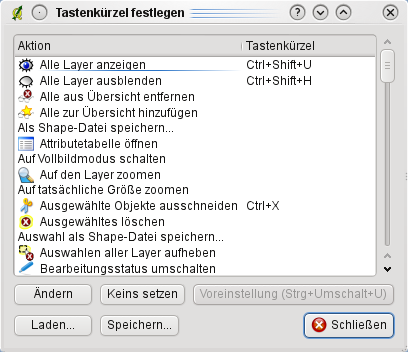
\includegraphics[clip=true, width=8cm]{shortcuts}
   \caption{Fenêtre de configuration des raccourcis \nixcaption (KDE)} \label{fig:shortcuts}
\end{figure}

La configuration est très simple. Sélectionnez une action dans la liste et cliquez sur le bouton \button{Changement}, \button{Mettre rien} ou \button{Définir par défaut}. Lorsque vous êtes satisfait de votre configuration, vous pouvez la sauver dans un fichier xml en vue de  charger ce dernier dans un autre environnement d'exécution de \qg (sur un autre ordinateur par exemple). 

\subsection{Aide contextuelle} \label{context_help}
%\index{Context help}
\index{Aide contextuelle}

Lorsque le besoin d'aide se fait sentir sur un sujet spécifique, vous pouvez accéder à l'aide contextuelle via le bouton d'aide disponible dans la plupart des fenêtres de dialogue — veuillez noter que les extensions additionnelles peuvent pointer vers des pages web dédiées.

\section{Rendu} \label{subsec:redraw_events} \index{rendu}

Par défaut, \qg effectue le rendu de toutes les couches visibles à chaque fois que l'affichage de la carte a besoin d'être mis à jour. Les évènements qui déclenchent ce rafraîchissement incluent :

\begin{itemize}[label=--]
\item l'ajout d'une couche,
\item un déplacement ou un zoom,
\item un redimensionnement de la fenêtre de \qg,
\item le changement d'état de visibilité d'une couche.
\end{itemize}

\qg vous laisse contrôler le processus de rendu de plusieurs manières.

\subsection{Rendu dépendant de l'échelle} \index{rendu!dépendant de l'échelle}
\label{label_scaledepend}

Le rendu dépendant de l'échelle permet de spécifier les échelles minimale et maximale auxquelles la couche doit être visible. Pour définir une échelle de rendu, ouvrez la fenêtre de \dialog{Propriétés} en double-cliquant sur une couche dans la légende et dans l'onglet \tab{Général}, saisissez les valeurs voulues puis cochez la case \checkbox{Utiliser le rendu dépendant de la mise à l'échelle}.

Vous pouvez déterminer les valeurs d'échelle en zoomant au niveau que vous voulez utiliser et en notant les valeurs de la barre d'état.\index{échelle}

\subsection{Contrôler le rendu} \label{label_controlmap}

Le rendu de la carte peut être contrôlé de différentes manières :

\minisec{a) Suspendre le rendu} \index{rendu!suspendre}
\label{label_suspendrender}

Pour suspendre le rendu, cliquez sur la case \checkbox{Rendu}dans le coin inférieur droit de la barre de statut. Quand cette case n'est pas cochée, \qg ne redessine pas la carte en réponse aux évènements décrits dans la section \ref{subsec:redraw_events}. Voici quelques cas pour lesquels vous pourriez souhaiter ce comportement :

\begin{itemize}[label=--]
\item l'ajout d'un nombre important de couches et la définition de la sémiologie avant d'effectuer un rendu potentiellement long,
\item l'ajout d'une ou plusieurs couches et le changement d'échelle,
\item l'ajout d'une ou plusieurs couches et le zoom sur un endroit spécifique,
\item n'importe quelle combinaison des éléments précédents.
\end{itemize}

Cocher la case \checkbox{Rendu} activera de nouveau le rendu et provoquera un rafraîchissement immédiat de la vue active.

\minisec{b) Définir les options d'ajout de couche} \label{label_settinglayer}
\index{rendu!options} \index{couche!visibilité intitiale}

Il est possible de définir une option qui chargera toutes les nouvelles couches sans les dessiner, elles seront ajoutées à la carte, mais la case de visibilité sera décochée par défaut. Pour définir cette option, sélectionnez l'option \mainmenuopt{Préférences} > \dropmenuopt{Options} et cliquez sur l'onglet \tab{Rendu et SVG}. Décochez la case \checkbox{par défaut les couches supplémentaires sont affichées}. Les nouvelles couches ajoutées à la carte seront invisibles par défaut.

%\minisec{Arrêter le rendu} \index{rendering!halting}
%\label{label_stoprender}
%
%Pour arrêter le rendu de la carte, appuyez sur la touche ESC. Ceci stoppera le rafraîchissement de la vue de la carte et laissera la carte partiellement dessinée. Il est possible qu'il y ait un délai entre le moment où la touche est pressée et le moment où le rendu de la carte est effectivement arrêté.
%
%\textbf{NOTE}: Il n'est pas actuellement possible d'arrêter le rendu de cette manière — cette fonctionnalité a été désactivée lors du port vers qt4 du fait d'instabilités.
%
\minisec{c) Mettre à jour l'affichage de la carte pendant le rendu de l'affichage}
\label{label_updatemap} \index{rendu!mise à jour de l'affichage}

Vous pouvez définir une option pour mettre à jour l'affichage de la carte quand des entités sont dessinées. Par défaut, \qg n'affiche pas les entités d'une couche tant que la couche entière n'a pas été rendue. Pour mettre à jour l'affichage à mesure que les entités sont lues dans la table attributaire, sélectionnez le menu \mainmenuopt{Préférences} > \dropmenuopt{Options} puis l'onglet \tab{Rendu et SVG}. Mettez comme valeur le nombre d'entités à mettre à jour durant le rendu. Si elle est égale à 0, cela désactive la mise à jour durant le dessin (c'est la valeur par défaut). Une valeur trop basse risque d'impacter les performances, car la vue de la carte sera constamment mise à jour durant la lecture des entités. Il est suggéré de commencer à 500.

\minisec{d) Influencer la qualité du rendu}
\label{label_renderquality} \index{rendu!qualité}

Pour influencer la qualité du rendu de la carte vous avez trois possibilités. Dans le menu \mainmenuopt{Préférences} > \dropmenuopt{Options} puis l'onglet \tab{Rendu et SVG} et sélectionnez/désélectionnez les cases suivantes :
\begin{itemize}[label=--]
\item \checkbox{Les lignes semblent moins déchiquetées aux dépens d'une certaine vitesse d'exécution}
\item \checkbox{Corriger les polygones remplis de manière erronée}
%\item \checkbox{Rafraîchir en permanence lors du déplacement de la table des matières/carte}
\end{itemize}

\section{Mesurer} \label{sec:measure} \index{mesure}

Les mesures fonctionnent uniquement au sein des systèmes de coordonnées projetées (exemple : UTM, Lambert 93). Si la couche active est définie par un système géographique de coordonnées (latitude/longitude), les résultats d'une mesure de ligne ou d'aires seront incorrects. Pour y remédier, vous devez spécifier un système de coordonnées plus approprié (voir Section~\ref{label_projections}). Les deux outils de mesure peuvent utiliser les paramètres d'accrochage de l'outil de numérisation. C'est utile pour mesurer des distances et des aires pour des couches vectorielles.

Pour sélectionner un outil de mesure, cliquez sur 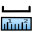
\includegraphics[width=0.7cm]{mActionMeasure} puis sur l'outil voulu.

\subsection{Mesurer une longueur, une aire et un angle}
\index{mesure!longueur}
\index{mesure!aires}
\index{mesure!angles}

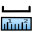
\includegraphics[width=0.7cm]{mActionMeasure} 
\qg peut mesurer des distances réelles entre plusieurs points selon un ellipsoïde défini. Pour le configurer, allez dans le menu \mainmenuopt{Préférences} > \dropmenuopt{Options}puis dans l'onglet \tab{Outils cartographiques} et choisissez l'ellipsoïde approprié. Vous pouvez également modifier ici la couleur du trait et l'unité de mesure (mètre ou pied). Cet outil permet de placer des points sur la carte. La longueur de chaque segment s'affiche dans la fenêtre de mesure ainsi que la longueur cumulée totale. Pour stopper les mesures, faites un clic droit. \par
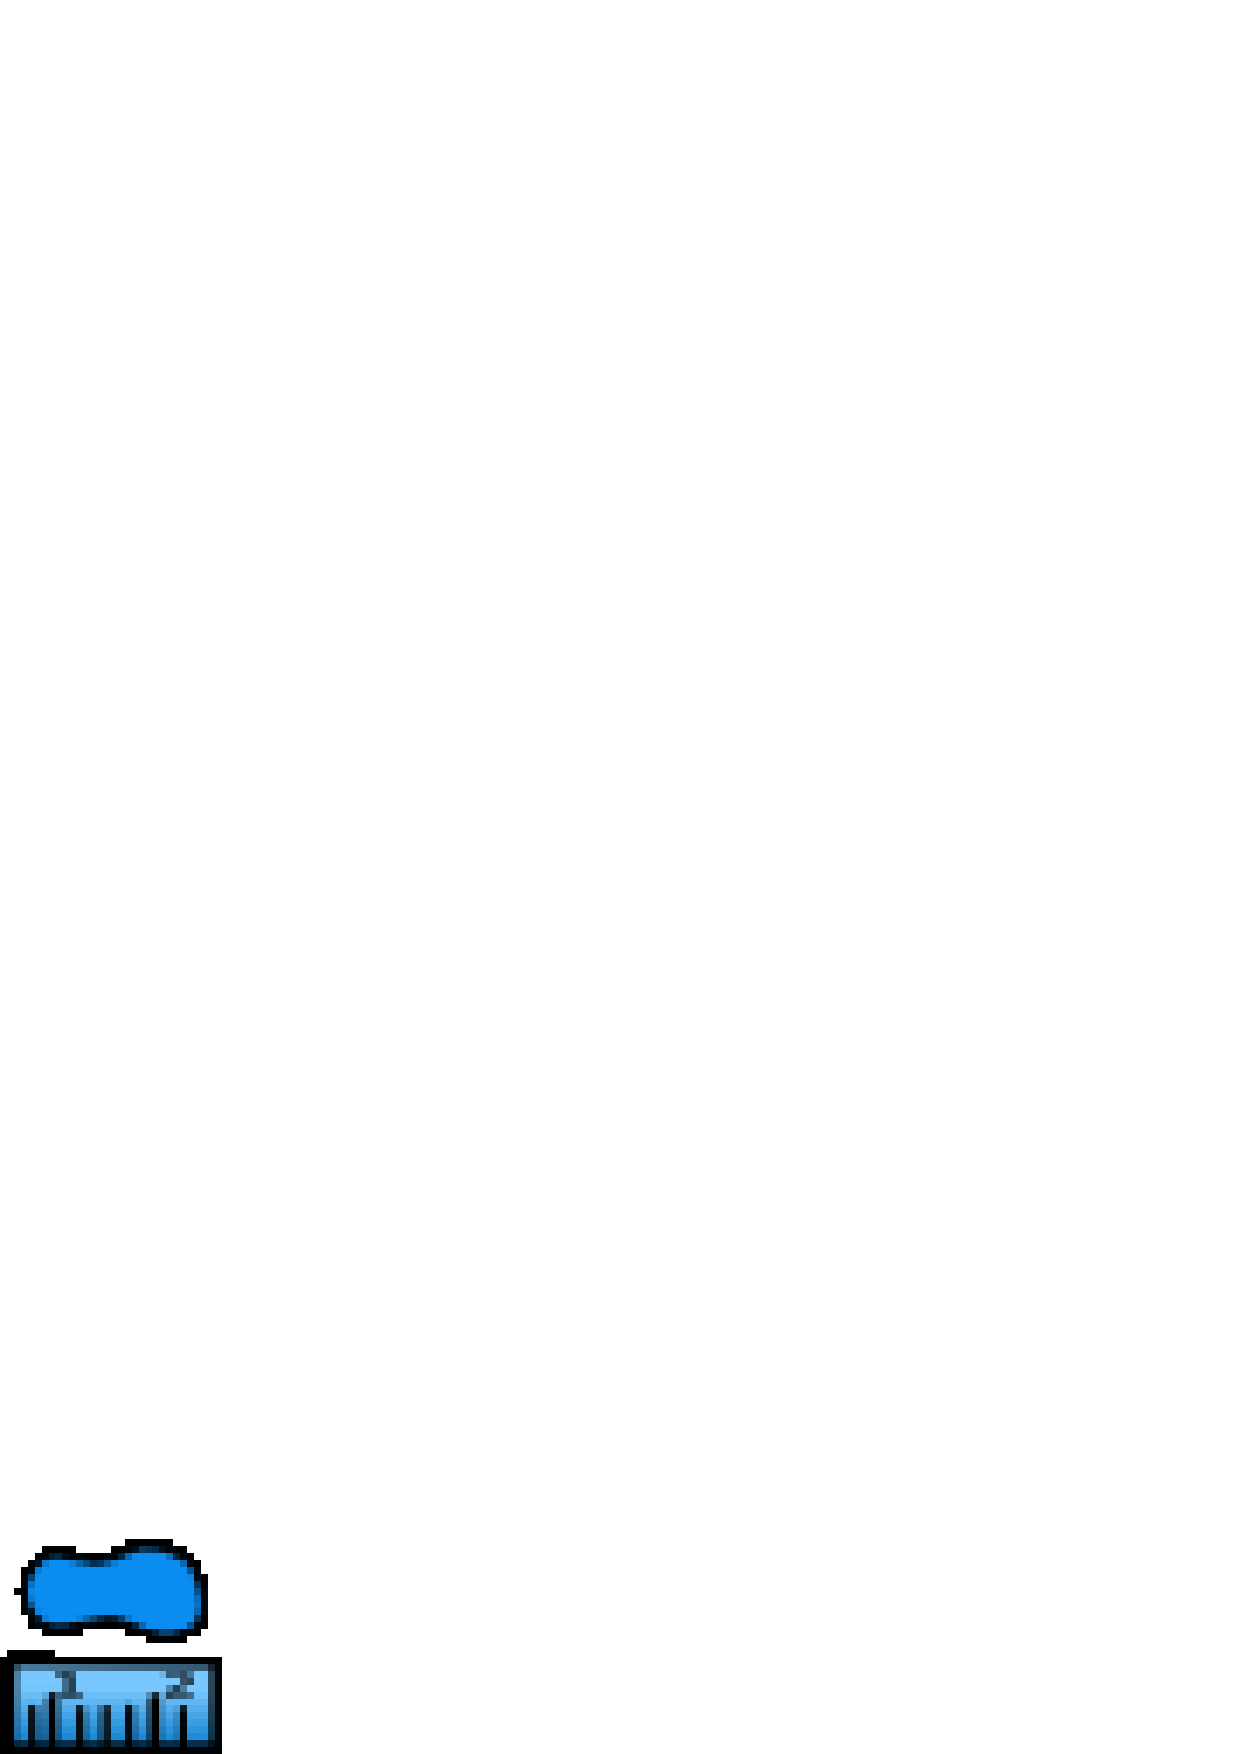
\includegraphics[width=0.7cm]{mActionMeasureArea} Les aires peuvent aussi être mesurées.
Dans la fenêtre de mesure apparaît la surface totale mesurée. \par
En complément, l'outil de mesure s'accrochera à la couche sélectionnée à partir du moment où celle-ci à un seuil d'accrochage défini (voir la section \ref{snapping_tolerance}). Donc si vous voulez mesurer avec exactitude une ligne ou le contour d'un polygone, spécifiez d'abord un seuil d'accrochage puis sélectionnez la couche. Avec l'outil de mesure, chaque clic de souris se situant dans ce seuil s'accrochera aux entités de cette couche. \par
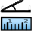
\includegraphics[width=0.7cm]{mActionMeasureAngle}
Vous pouvez aussi mesurer des angles en sélectionnant l'outil de mesure d'angles. Le curseur adopte une forme en croix. Cliquez pour dessiner le premier côté de l'angle à mesurer puis bouger le curseur pour dessiner l'angle désiré. La mesure est affichée dans une fenêtre de dialogue.

\begin{figure}[ht]
\centering
  \subfloat[Mesure de distances] {\label{subfig:measure_line} 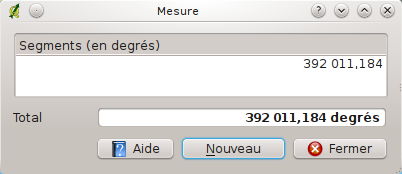
\includegraphics[clip=true, width=0.3\textwidth]{measure_line}}
  \hspace{0.5cm}
  \subfloat[Mesure d'aires]{\label{subfig:measure_area} 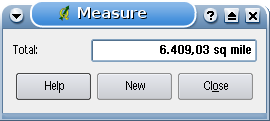
\includegraphics[clip=true, width=0.3\textwidth]{measure_area}}
  \hspace{0.5cm}
  \subfloat[Mesure d'angles]{\label{subfig:measure_angle} 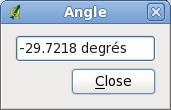
\includegraphics[clip=true, width=0.15\textwidth]{measure_angle}}
  \caption{Outils de mesure \nixcaption} \label{fig:measure}
\end{figure}

%\subsection{Select and deselect features}\label{sec:selection}
\subsection{Sélectionner et désélectionner des entités}\label{sec:selection}

%The QGIS toolbar provides several tools to select features in the map canvas. 
%To select one or several features just click on 
%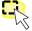
\includegraphics[width=0.7cm]{mActionSelect} and select the tools:
La barre d'outils fournit plusieurs outils de sélection d'entités à partir du canevas de la carte. pour sélectionner une ou plusieurs entités, cliquez  sur 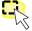
\includegraphics[width=0.7cm]{mActionSelect}\footnote{Un clic plus long ou un clic sur la flèche noir pointée vers le bas suffiront.} et choisissez l'outil :

\begin{description}
%\item \radiobuttonon{Select features}
\item \radiobuttonon{Sélection d'entités}
%\item \radiobuttonoff{Select features by rectangle}
\item \radiobuttonoff{Sélection d'entités avec un rectangle}
%\item \radiobuttonoff{Select features by polygon}
\item \radiobuttonoff{Sélection d'entités avec un polygone}
%\item \radiobuttonoff{Select features by freehand}
\item \radiobuttonoff{Sélection d'entités à main levée}
%\item \radiobuttonoff{Select features by radius}
\item \radiobuttonoff{Sélection d'entités selon un rayon}
\end{description} 

Pour désélectionner toutes les entités, cliquez sur 
\includegraphics[width=0.7cm]{mActionDeselectAll}.

\section{Les projets} \label{sec:projects} \index{projets}

L'état de votre session de \qg est considéré comme étant un projet. \qg ne peut travailler que sur un projet à la fois. Les propriétés sont considérées comme étant assignées à un projet ou celles par défaut des nouveaux projets (voir Section \ref{subsec:gui_options}). \qg peut enregistrer l'état de votre travail dans un fichier de projet en utilisant le menu \mainmenuopt{Fichier} > \dropmenuopttwo{mActionFileSave}{Sauvegarder le projet} ou \mainmenuopt{Fichier} > \dropmenuopttwo{mActionFileSaveAs}{Sauvegarder le projet sous...}. À la fermeture du projet (arrêt du logiciel ou ouverture, création d'un autre projet), le logiciel peut proposer l'enregistrement si l'état courant diffère de l'état enregistré. Pour activer cette option, rendez-vous dans l'onglet \tab{Général} du menu \mainmenuopt{Préférences} > \dropmenuopt{Options} et sélectionnez\\
\checkbox{\small Demander à sauvegarder si des changements ont été apportés au projet \qg}.

Pour charger un projet dans une session \qg, aller dans \mainmenuopt{Fichier} > \dropmenuopttwo{mActionFileOpen}{Ouvrir un Projet} ou \mainmenuopt{Fichier} > \dropmenuopt{Ouvrir un projet récent}. Si vous souhaitez revenir à une session vierge, aller sur \mainmenuopt{Fichier} > \dropmenuopttwo{mActionFileNew}{Nouveau Projet}.
Chacune de ces options vous demandera si vous désirez enregistrer le projet dès lors que des changements auront été effectués depuis son ouverture ou sa dernière sauvegarde.

Les types d'informations enregistrées dans un projet sont :

\begin{itemize}[label=--]
\item les couches ajoutées,
\item les propriétés des couches comprenant notamment la sémiologie,
\item la projection de la carte,
\item l'étendue de la dernière zone de visualisation.
\end{itemize}

Le fichier de projet est enregistré au format XML, il est donc possible de l'éditer en dehors de \qg si vous savez ce que vous faites. Le format a été modifié à plusieurs reprises depuis les versions antérieures de \qg, les fichiers enregistrés sous ces versions peuvent ne plus fonctionner correctement avec les versions ultérieures. Pour être averti dans ce genre de cas, allez dans l'onglet \tab{Général} du menu \mainmenuopt{Préférences} > \dropmenuopt{Options} et sélectionnez\\
\checkbox{\small M'avertir lors de l'ouverture d'un fichier projet sauvegardé avec une version précédente de \qg}.

\minisec{Propriétés de projet}
Dans la fenêtre de propriétés du projet vous pouvez mettre des options spécifiques à un projet. Cela inclut :
\begin{itemize}[label=--]
 \item Dans l'onglet \tab{Général} le titre du projet, les unités, et la possibilité d'enregistrer des chemins relatifs vers les couches. L'édition topologique et les options d'accrochage peuvent être changées ici.
\item L'onglet \tab{Système de Coordonnées de Référence (SCR)} permet de choisir le système de coordonnées pour ce projet et d'activer la projection à la volée des couches vectorielles utilisant un SCR différent.
\item Avec le troisième onglet \tab{Identification des couches} vous pouvez activer (ou désactiver) les couches qui répondront à l'outil d'identification (voir le paragraphe sur les outils de la carte dans la section \ref{subsec:gui_options}).
\end{itemize}

\section{Sortie graphique} \label{sec:output}
\index{export!enregistrer en tant qu'image!composeur de carte!impression rapide}

Plusieurs sorties graphiques sont possibles depuis votre session. Nous en avons déjà vue une dans la section \ref{sec:projects} : sauvegarder dans un fichier de projet.
Voici d'autres manières de produire une sortie graphique :
\begin{itemize}[label=--]
\item Menu option \dropmenuopttwo{mActionSaveMapAsImage}{Sauvegarder comme image...} ouvre une fenêtre de dialogue où vous devez saisir le nom, le chemin et le type d'image (PNG, JPEG, etc). Un fichier "worldfile" avec le même nom et la même extension à laquelle est ajoutée la lettre w (pngw, jpgw, etc), enregistré dans le même dossier que l'image, géoréférence celle-ci.
\item Menu option \dropmenuopttwo{mActionFilePrint}{Composeur d'impression} ouvre une fenêtre de dialogue où vous pouvez faire une mise en page et imprimer la vue active de la carte (voir Section~\ref{label_printcomposer})
\item L'extension \toolbtntwo{quick_print}{Impression rapide} permet de produire un fichier PDF à partir de la carte à moindres efforts (voir Section \ref{quickprint}).
\end{itemize}

\section{Options de l'interface graphique} \label{subsec:gui_options}

\includegraphics[width=0.7cm,clip=true]{mActionOptions} 
Quelques options basiques peuvent être sélectionnées en allant dans le menu \mainmenuopt{Préférences} >
\dropmenuopttwo{mActionOptions}{Options}. Les onglets dans lesquels vous pouvez configurer les options sont :

\minisec{Onglet Général}

\begin{itemize}[label=--]
\item \checkbox{Demander à sauvegarder les changements apportés au projet si requis}
\item \checkbox{\small M'avertir lors de l'ouverture d'un fichier projet sauvegardé avec une version précédente de \qg}
\item Changer les couleurs de sélection et de fond
\item Changer le thème des icônes (choix possible entre default, classic, gis et newgis)
\item \checkbox{Mettre les noms de couche en majuscules dans la légende}
\item \checkbox{Afficher les noms des attributs de classification dans la légende}
\item \checkbox{Créer les vignettes des rasters dans la légende}
\item \checkbox{Cacher l'écran de démarrage}
\item \checkbox{Ouvrir les résultats identifiés dans une fenêtre ancrable (redémarrage requis)}
\item \checkbox{Ouvrir la table d'attributs dans une fenêtre ancrable}
\item \checkbox{Ajouter une couche PostGIS avec un double-clic et sélectionner en mode étendu}
\item \checkbox{Ajouter les nouvelles couches au groupe sélectionné}
\item Définir le comportement de la table d'attributs (choisir entre montrer toutes les entités, celles sélectionnées et celles présentes dans la vue active)
\end{itemize}

\minisec{Onglet Rendu et SVG}

\begin{itemize}[label=--]
\item \checkbox{par défaut les couches ajoutées sont affichées}
\item Définir le nombre d'entités à dessiner avant d'actualiser l'affichage
\item \checkbox{Utiliser le cache de rendu, si possible, pour accélérer le rafraîchissement}
\item \checkbox{\small Les lignes semblent moins déchiquetées aux dépens d'une certaine vitesse d'exécution}
\item \checkbox{Corriger les polygones remplis de manière erronée}
\item \checkbox{Utiliser le moteur de rendu de sémiologie de nouvelle génération}
\item Modifier la liste des emplacements de recherche pour les symboles au format Scalable Vector Graphics (SVG)

En outre, vous pouvez choisir de sauver l'emplacement relatif ou absolu des textures SVG dans l'onglet \tab{Général} du menu \mainmenuopt{Préférences} > \dropmenuopttwo{mActionOptions}{Propriétés du projet}
%\item \checkbox{Rafraîchir en permanence la table des matières/carte lors du déplacement} 
\end{itemize}

\minisec{Onglet des Outils Cartographiques}

\begin{itemize}[label=--]
\item Le paramètre Mode détermine quelles couches seront prises en compte par l'outil d'identification. En choisissant \usertext{De haut en bas} ou \usertext{De haut en bas, s'arrêter au premier} à la place de \usertext{Couche sélectionnée}, les attributs de toutes les couches identifiables (voir la section sur les propriétés du projet \ref{sec:projects} pour sélectionner les couches identifiables) seront affichés par l'outil d'identification.
\item \checkbox{Ouvrir le formulaire d'entité si un seul objet est identifié}
\item Spécifier le rayon de recherche comme pourcentage de la largeur de la carte)
\item Définir l'ellipsoïde pour des calculs de distance
\item Définir la couleur du trait pour les outils de mesure
\item \radiobuttonon{Définir l'unité de mesure des distances (mètre ou pied}
\item \radiobuttonon{Définir l'unité de mesure des angles (degré, radian ou gon}
\item Définir l'action de la molette de la souris (Zoomer, Zoomer et récentrer, Zoomer sur le curseur de la souris, Rien)
\item Définir le facteur de zoom
\end{itemize}

\minisec{Revêtement}

\begin{itemize}[label=--]
\item Définir l'algorithme de placement des étiquettes (choisir entre le point central (par défaut), Chaîne, Chaîne popmusic tabu, popmusic tabu et Chaîne popmusic)
\end{itemize}

\minisec{Onglet de Numérisation}

\begin{itemize}[label=--]
\item Définir la couleur et la largeur de la ligne d'étirement
\item Définir le mode d'accrochage par défaut (à un sommet, un segment, aux sommets et segments)
\item Définir la tolérance d'accrochage par défaut (en unités de la carte ou en pixels) 
\item Définir le rayon de recherche pour l'édition des sommets (en unités de la carte ou en pixels)
\item \checkbox{Montrer les marqueurs seulement pour les entités sélectionnées}
\item Définir l'aspect des marqueurs de sommet (croix, cercle semi-transparent ou pas de symbole) et leur taille.
\item \checkbox{Supprimer la fenêtre d'attributs apparaissant après chaque création d'entité}
\end{itemize}

\minisec{Onglet de SCR}

\begin{itemize}[label=--]
\item \radiobuttonoff{Demander pour le Système de Coordonnées de Référence (SCR)}
\item \radiobuttonoff{Employer la projection globale par défaut du projet}
\item \radiobuttonon{Employer la projection par défaut ci-dessous}
\item Sélectionner le Système de Coordonnées de Référence (SCR) par défaut
\end{itemize}

\minisec{Onglet de Paramètres du lieu}

\begin{itemize}[label=--]
\item \checkbox{Forcer les paramètres linguistiques}
\item Paramètres de lieu sur votre système
\end{itemize}

\minisec{Onglet Réseau et Proxy}
{\setlength{\baselineskip}{1.4\baselineskip}
\begin{itemize}[label=--]
\item \checkbox{Utiliser un proxy pour l'accès internet}, définition de l'hôte, du port, de l'utilisateur et du mot de passe.
\item Modifiez le \dropmenuopt{type de Proxy} selon vos besoins
 \begin{itemize}[label=--,itemsep=2pt]
  \item \dropmenuopt{Proxy par défaut}: ce proxy est déterminé en se basant sur le proxy de l'application
  \item \dropmenuopt{Socks5Proxy}: proxy générique pour n'importe quel type de connexion. Supporte TCP, UDP, le lien à un port (pour les connexions entrantes) et l'authentication
  \item \dropmenuopt{HttpProxy}: utilise la commande CONNECT, supporte seulement les connexions TCP sortantes et l'authentification
  \item \dropmenuopt{HttpCachingProxy}: utilise les commandes normales HTTP, c'est utile uniquement dans le contexte de requête HTTP
  \item \dropmenuopt{FtpCachingProxy}: utilise un proxy FTP, ce n'est utile que dans le cas de requête FTP
\end{itemize}
\item Répertoire et taille du cache
\item Adresse de recherche WMS
\item \checkbox{Définir le délai d'abandon des requêtes en ms}
\end{itemize}}

L'exclusion d'adresses peut être ajoutée dans la boîte de texte en dessous des paramètres de proxy (voir fig. \ref{fig:proxy-settings}) en pressant le bouton \button{Ajouter}. Ensuite double-cliquer sur l'URL nouvellement créée est entrer l'adresse que vous voudriez exclure du proxy. Le bouton \button{Supprimer} efface l'entrée sélectionnée.

Si vous désirez des informations plus détaillées sur les différents paramètres, veuillez vous référer au manuel de la bibliothèque Qt à \url{http://doc.trolltech.com/4.5/qnetworkproxy.html#ProxyType-enum}.

\begin{figure}[ht]
   \begin{center}
   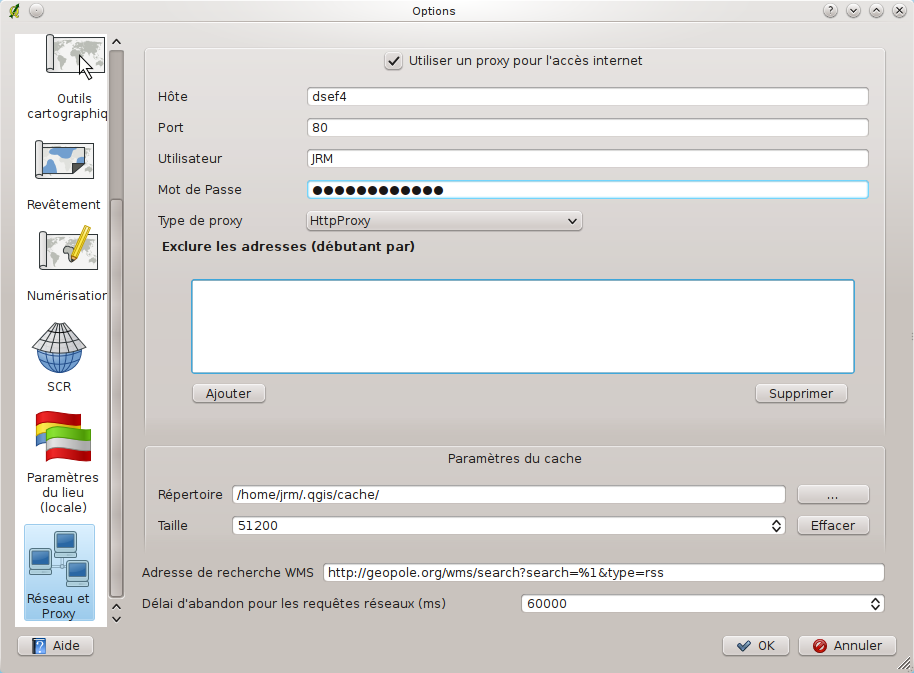
\includegraphics[clip=true, width=10cm]{proxy-settings}
   \caption{Paramétrer un proxy \nixcaption}
   \label{fig:proxy-settings}
\end{center} 
\end{figure}

\begin{Tip} \caption{\textsc{Utiliser un proxy}}
Utiliser un serveur mandataire (proxy) peut être compliqué, vous pouvez multiplier les essais et erreurs en cochant les cases jusqu'à obtenir une connexion qui vous satisfasse.
\end{Tip}

Vous pouvez modifier ces options selon vos besoins, certains de ces changements nécessiteront un redémarrage avant d'être effectifs.

\begin{itemize}[label=--]
\item \nix{les paramètres sont enregistrés dans un fichier texte:\\ \$HOME/.config/QuantumGIS/qgis.conf}
\item \osx{les paramètres sont enregistrés dans: \$HOME/Library/Preferences/org.qgis.qgis.plist}
\item \win{les paramètres sont enregistrés dans le registre sous:}
\begin{verbatim}
\\HKEY\CURRENT\USER\Software\QuantumGIS\qgis
\end{verbatim}
\end{itemize}

\section{Outils d'annotation} \label{sec:annotations}
\index{annotations}
\index{annotation de texte}

L'outil d'annotation 
\includegraphics[width=0.7cm, clip=true]{mActionTextAnnotation} dans la barre d'outils d'attribut fournit la possibilité de placer du texte formaté dans des phylactères sur la carte. Sélectionnez l'outil d'annotation puis cliquez sur la carte. Cette action place un marqueur à l'endroit du clic et un phylactère associé.

\begin{figure}[ht]
   \centering
   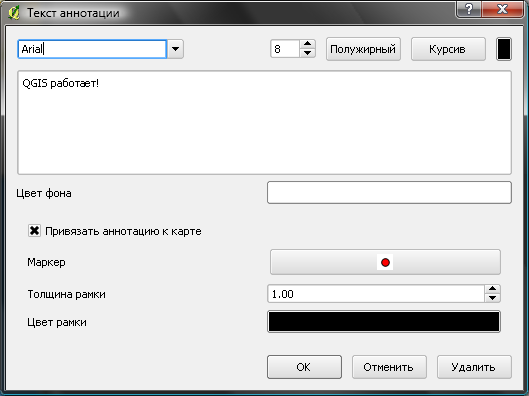
\includegraphics[clip=true, width=10cm]{annotation}
   \caption{fenêtre de dialogue de l'outil d'annotation \nixcaption}
   \label{fig:annotation}
\end{figure}

Un double clic dans l'emprise d'une annotation (matérialisée par quatre carrés aux angles) provoque l'ouverture d'une fenêtre de dialogue avec diverses options. Il y a un éditeur de texte avec quelques options (choix de la police de caractères, de la taille, de la graisse, etc.), le choix de la couleur de fond du cadre, ainsi que de la couleur et de l'épaisseur du contour. Il est également possible de choisir le marqueur. Ce dernier est affiché lorsque \checkbox{Position fixe de la carte} est activé : l'annotation est associée à un endroit de la carte et en suit les déplacements. Si l'option est désactivée, la position de l'annotation est relative à l'interface graphique et n'est pas impactée par la navigation dans la carte. La bulle peut être déplacée indépendamment du marqueur. Le déplacement du marqueur affecte l'ensemble de l'annotation.

L'outil 
\includegraphics[width=0.7cm,clip=true]{mActionAnnotation} Déplacer une annotation permet de déplacer l'annotation sur la carte.  

\minisec{Formulaire d'annotation} \index{annotations}
\index{annotation de formulaire}

En outre, vous pouvez créer vos propres formulaires d'annotation. L'outil 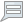
\includegraphics[width=0.7cm,clip=true]{mActionFormAnnotation} Formulaire d'annotation est utilisé pour afficher les attributs d'une entité dans un formulaire qt personnalisé (voir Figure \ref{fig:custom-annotations}). L'approche est similaire à la conception de formulaires pour l'outil d'identification, mais affiche les informations sous la forme d'une annotation. Pour un complément d'information, reportez-vous au blog \url{http://blog.qgis.org/node/143}.

\begin{figure}[ht]
   \centering
   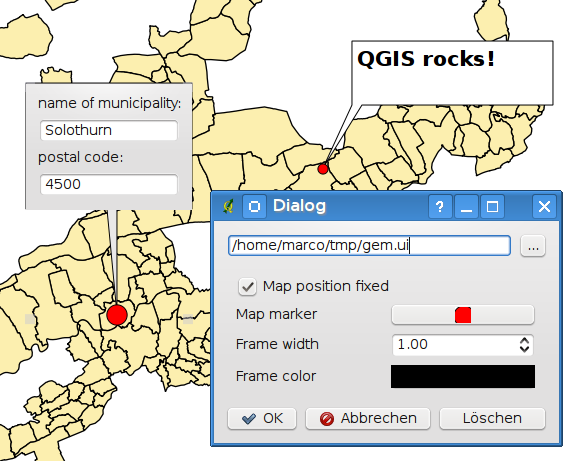
\includegraphics[clip=true, width=10cm]{custom_annotation}
   \caption{Formulaire d'annotation qt personnalisé \nixcaption}
   \label{fig:custom-annotations}
\end{figure}

\newpage


\section{Signets spatiaux} \label{sec:bookmarks}
\index{signets}
\index{signets spatiaux|\voir{signets}}

Les signets spatiaux vous permettent de marquer une zone de la carte pour y retourner plus tard.

\subsection{Créer un signet}
Pour créer un signet :
\begin{enumerate}
\item Déplacez-vous sur la zone concernée
\item Sélectionnez le menu \mainmenuopt{Vue} > \dropmenuopt{Nouveau signet} ou appuyez sur la touche \keystroke{Ctrl-B}
\item Entrez un nom pour décrire le signet (jusqu'à 255 caractères)
\item Cliquez sur \button{OK} pour ajouter le signet ou sur \button{Annuler} pour sortir de la fenêtre sans l'enregistrer
\end{enumerate}

Vous pouvez avoir plusieurs signets portant le même nom.

\subsection{Travailler avec les signets}
Pour utiliser ou gérer les signets allez dans le menu \mainmenuopt{Vue} > \dropmenuopt{Montrer les signets}.
Le dialogue \dialog{Signets géospatiaux} vous permet de rappeler ou d'effacer un signet.
Vous ne pouvez pas modifier le nom d'un signet ou ses coordonnées.

\subsection{Zoomer sur un signet}
Depuis la fenêtre \dialog{Signets géospatiaux}, sélectionnez le signet voulu en cliquant dessus puis sur le bouton \button{Zoomer sur}. Vous pouvez aussi zoomer en opérant un double-clic.

\subsection{Effacer un signet}
Pour effacer un signet depuis la fenêtre \dialog{Signets géospatiaux}, cliquez dessus puis sur le bouton \button{Effacer}.
Confirmez votre choix en cliquant sur \button{Oui} ou annuler en cliquant sur \button{Non}

\section{Suivi GPS en direct} \label{sec:gpstracking}

Pour activer le suivi GPS en direct dans \qg, vous devez sélectionner \mainmenuopt{Vue} > \dropmenuopt{Suivi GPS en direct}. Une nouvelle fenêtre sera ancrée à gauche de la carte.

Cette fenêtre propose quatre écrans différents (voir Figure \ref{fig:gpstrack_live} et Figure \ref{fig:gpstrack_options}).

\begin{description}
 \item[(a)] 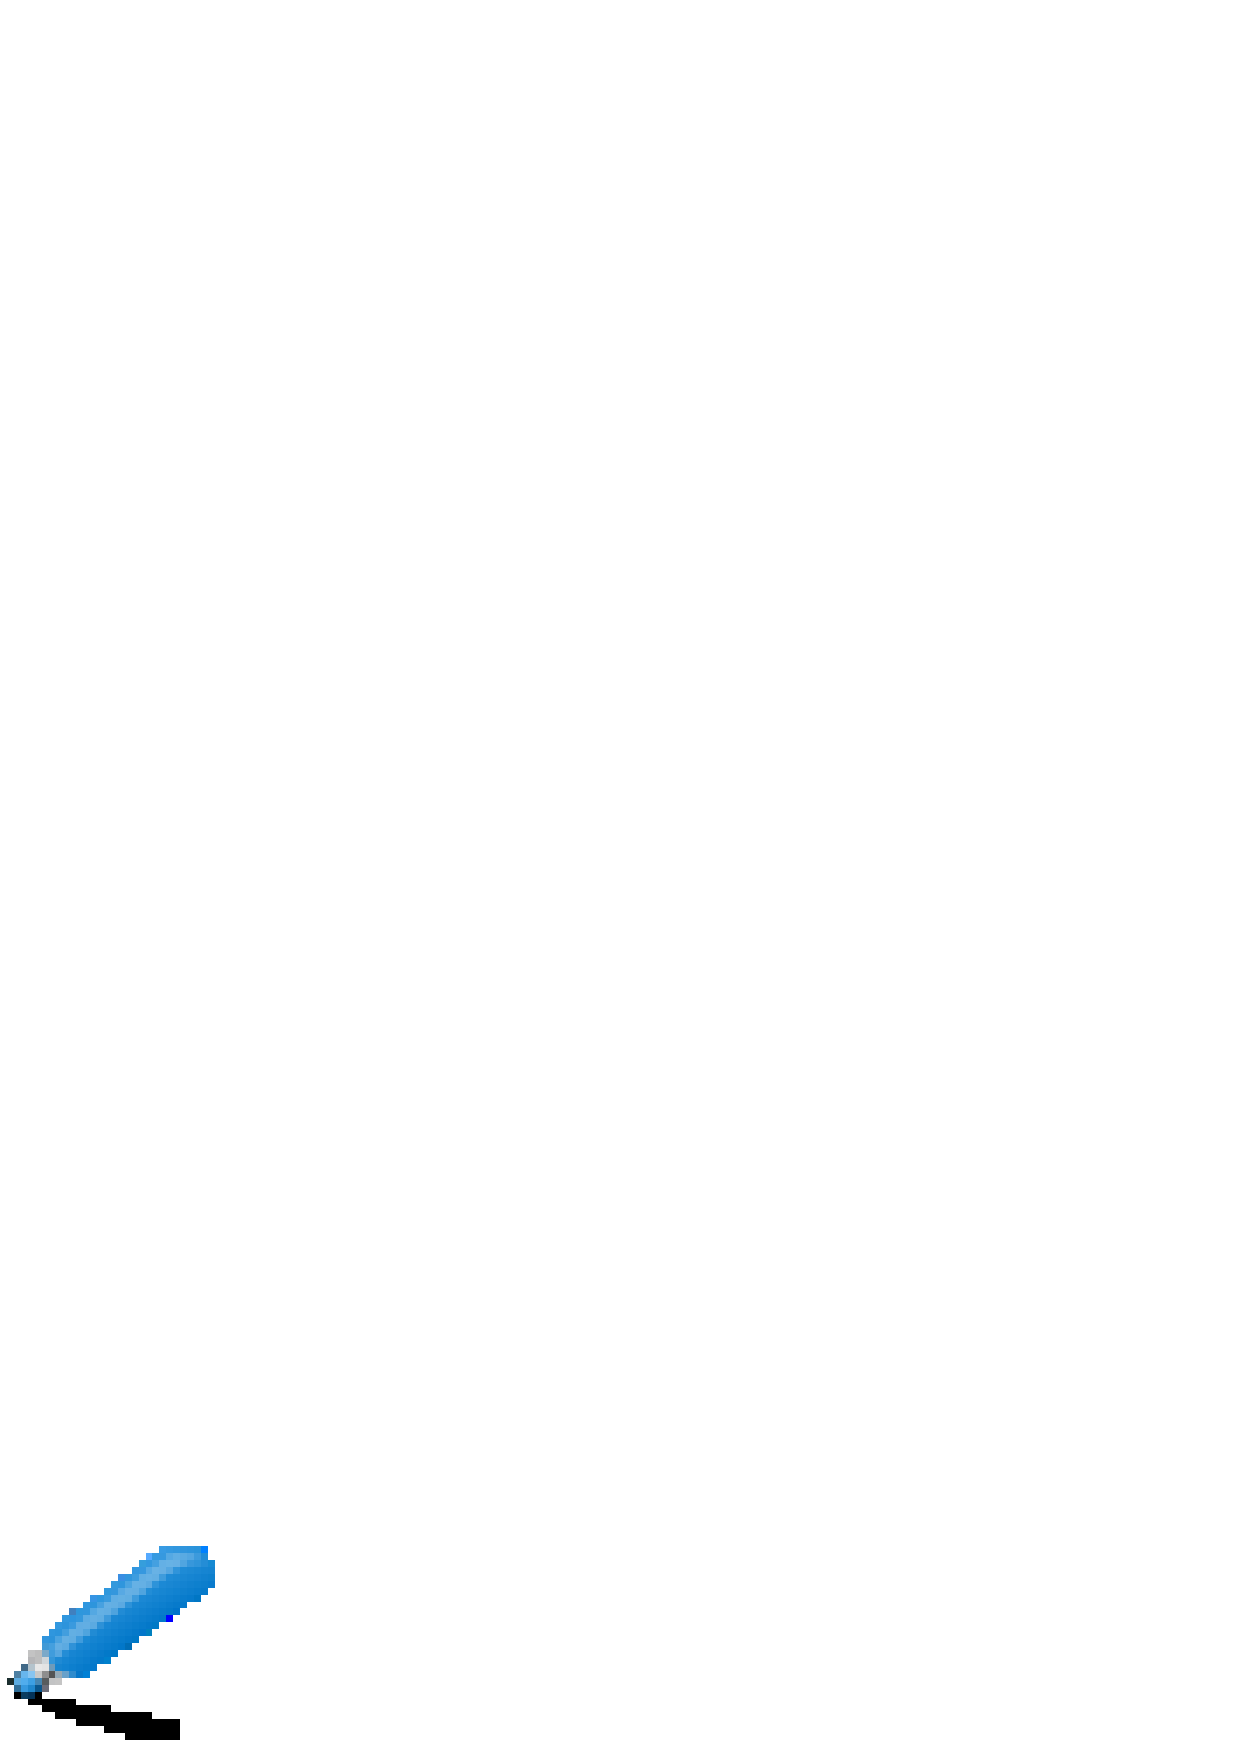
\includegraphics[width=0.5cm,clip=true]{mActionToggleEditing} 
Coordonnées de la position GPS et saisie manuelle de sommets et d'entités.
 \item[(b)] 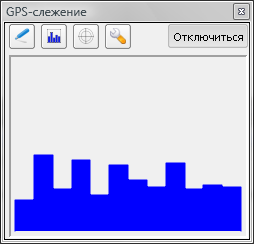
\includegraphics[width=0.5cm,clip=true]{gpstrack_barchart} 
Force des signaux GPS des satellites connectés. 
 \item[(c)] 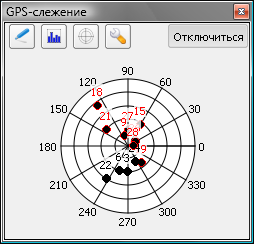
\includegraphics[width=0.5cm,clip=true]{gpstrack_polarchart} 
Graphe polaire montrant le numéro SV et la position des satellites. 
 \item[(d)] 
\includegraphics[width=0.5cm,clip=true]{mActionOptions} 
Écran des options GPD (voir Figure \ref{fig:gpstrack_options}).
\end{description}

Avec un récepteur GPS connecté (il doit être compatible avec votre système d'exploitation), un simple clic sur \button{Connexion} connecte le GPS à \qg. Un second clic (maintenant \button{Déconnexion}) déconnecte le récepteur de l'ordinateur. Sous GNU/Linux, le support gpsd est intégré afin de supporter la connexion de la majorité des récepteurs GPS. De ce fait, vous devez préalablement configurer gpsd pour y connecter \qg.

[ IMPORTANT ]: Si vous désirez enregistrer votre position sur la carte, vous devez, au préalable, créer une nouvelle couche et la passer en mode édition.

\begin{figure}[ht]
\centering
   \subfloat[Coordonnées de la position] {\label{subfig:gpstrack_main} 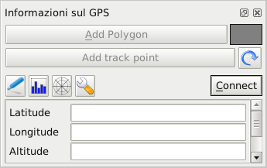
\includegraphics[clip=true, width=0.3\textwidth]{gpstrack_main}}
     \hspace{0.33cm}
   \subfloat[Force du signal GPS]{\label{subfig:gpstrack_stren} 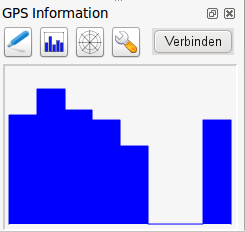
\includegraphics[clip=true, width=0.3\textwidth]{gpstrack_stren}}
     \hspace{0.33cm}
   \subfloat[Graphe polaire]{\label{subfig:gpstrack_polar} 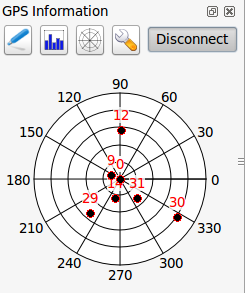
\includegraphics[clip=true, width=0.3\textwidth]{gpstrack_polar}}
\caption{Suivi GPS en direct \nixcaption} \label{fig:gpstrack_live}
\end{figure}

\begin{figure}[ht]
   \centering
   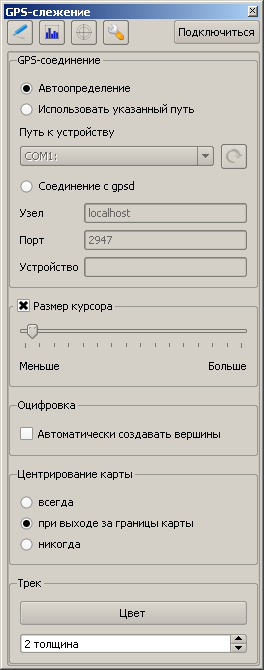
\includegraphics[clip=true, width=8cm]{gpstrack_options}
   \caption{Écran de configuration du suivi GPS \nixcaption}
   \label{fig:gpstrack_options}
\end{figure}

\subsection{Coordonnées de la position}
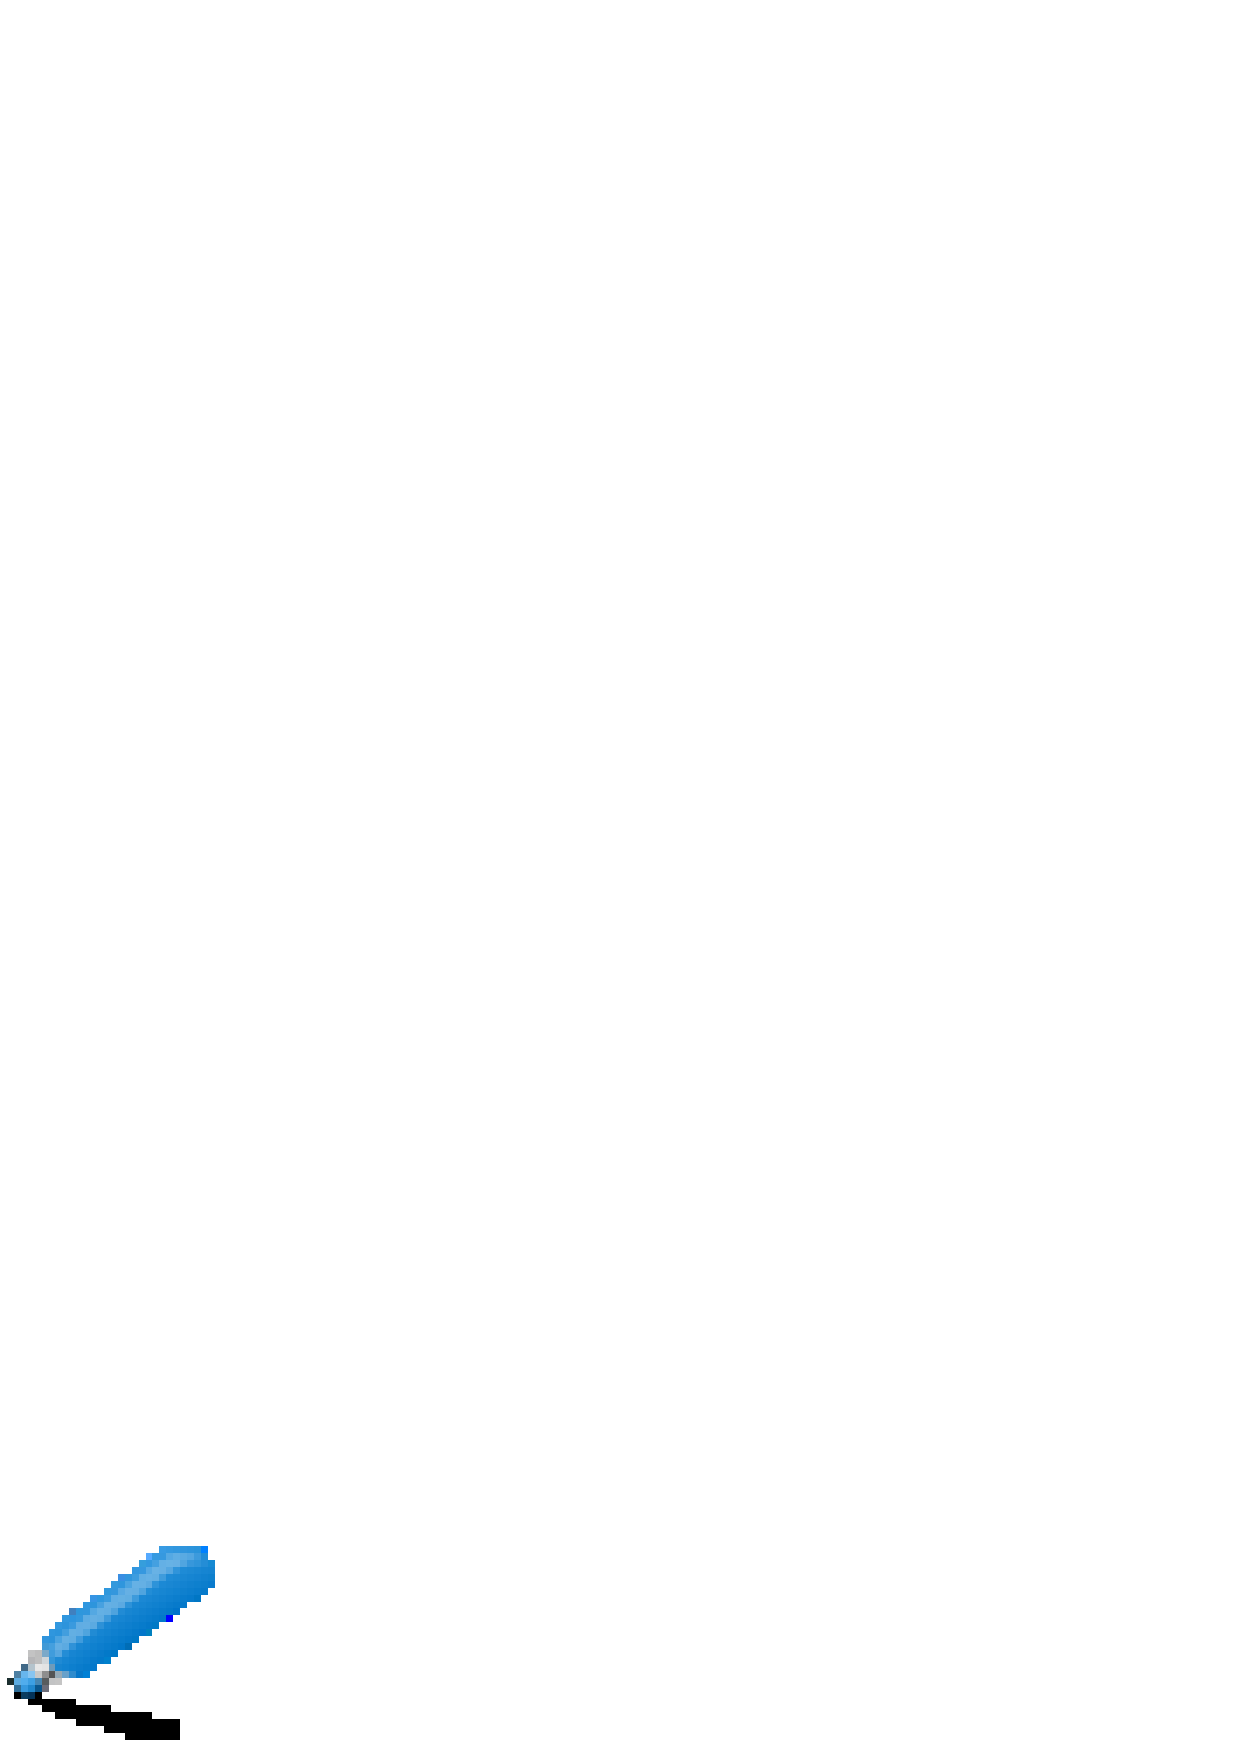
\includegraphics[width=0.5cm,clip=true]{mActionToggleEditing} Si le GPS reçoit les signaux d'un nombre suffisant de satellites, vous verrez votre position exprimée en latitude, longitude et élévation comme vous pouvez le voir sur la figure \ref{subfig:gpstrack_main}.

\subsection{Force du signal GPS}
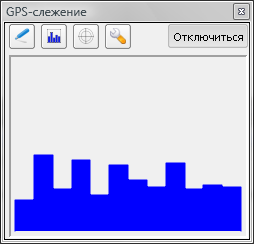
\includegraphics[width=0.5cm,clip=true]{gpstrack_barchart} Cet écran affiche la force des signaux GPS des satellites connectés sous forme de barres (Figure \ref{subfig:gpstrack_stren}).

\subsection{Graphe polaire}
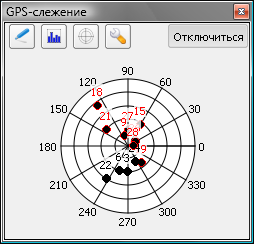
\includegraphics[width=0.5cm,clip=true]{gpstrack_polarchart} Si vous voulez connaître la position des satellites connectés, vous devez passer à l'écran du graphe polaire (Figure \ref{subfig:gpstrack_polar}).
Les satellites connectés sont identifiés par leur numéro PRN (Pseudo Random Number).

\subsection{Configuration GPS}

\includegraphics[width=0.5cm,clip=true]{mActionOptions} Si vous faites face à des problèmes de connexion, vous pouvez passer de \radiobuttonon{Autodétecter} à \radiobuttonon{Utiliser le chemin/port suivant} et sélectionnez le chemin, port auquel votre GPS est connecté. 
Un clic sur \button{Connexion} initialise à nouveau la connexion au récepteur GPS.

Avec la glissière \slider{Taille du curseur GPS} vous augmenter ou diminuer le curseur marquant la position sur la carte. En activant \radiobuttonon{Ajout automatique de sommets} dans la section numérisation GPS, votre parcours sera automatiquement enregistré dans la couche vectorielle active, à la condition qu'elle soit en mode édition. 

Dans la section recentrer la carte GPS, vous pouvez définir le critère de rafraîchissement de la carte lorsque votre position change : centrage de la carte sur votre position en continu, centrage lorsque le curseur quitte la zone affichée ou aucun changement. 

La section pister permet de sélectionner la couleur et la largeur de la ligne correspondant à votre parcours.

Si vous voulez enregistrer une entité manuellement, vous devez retourner à l'écran 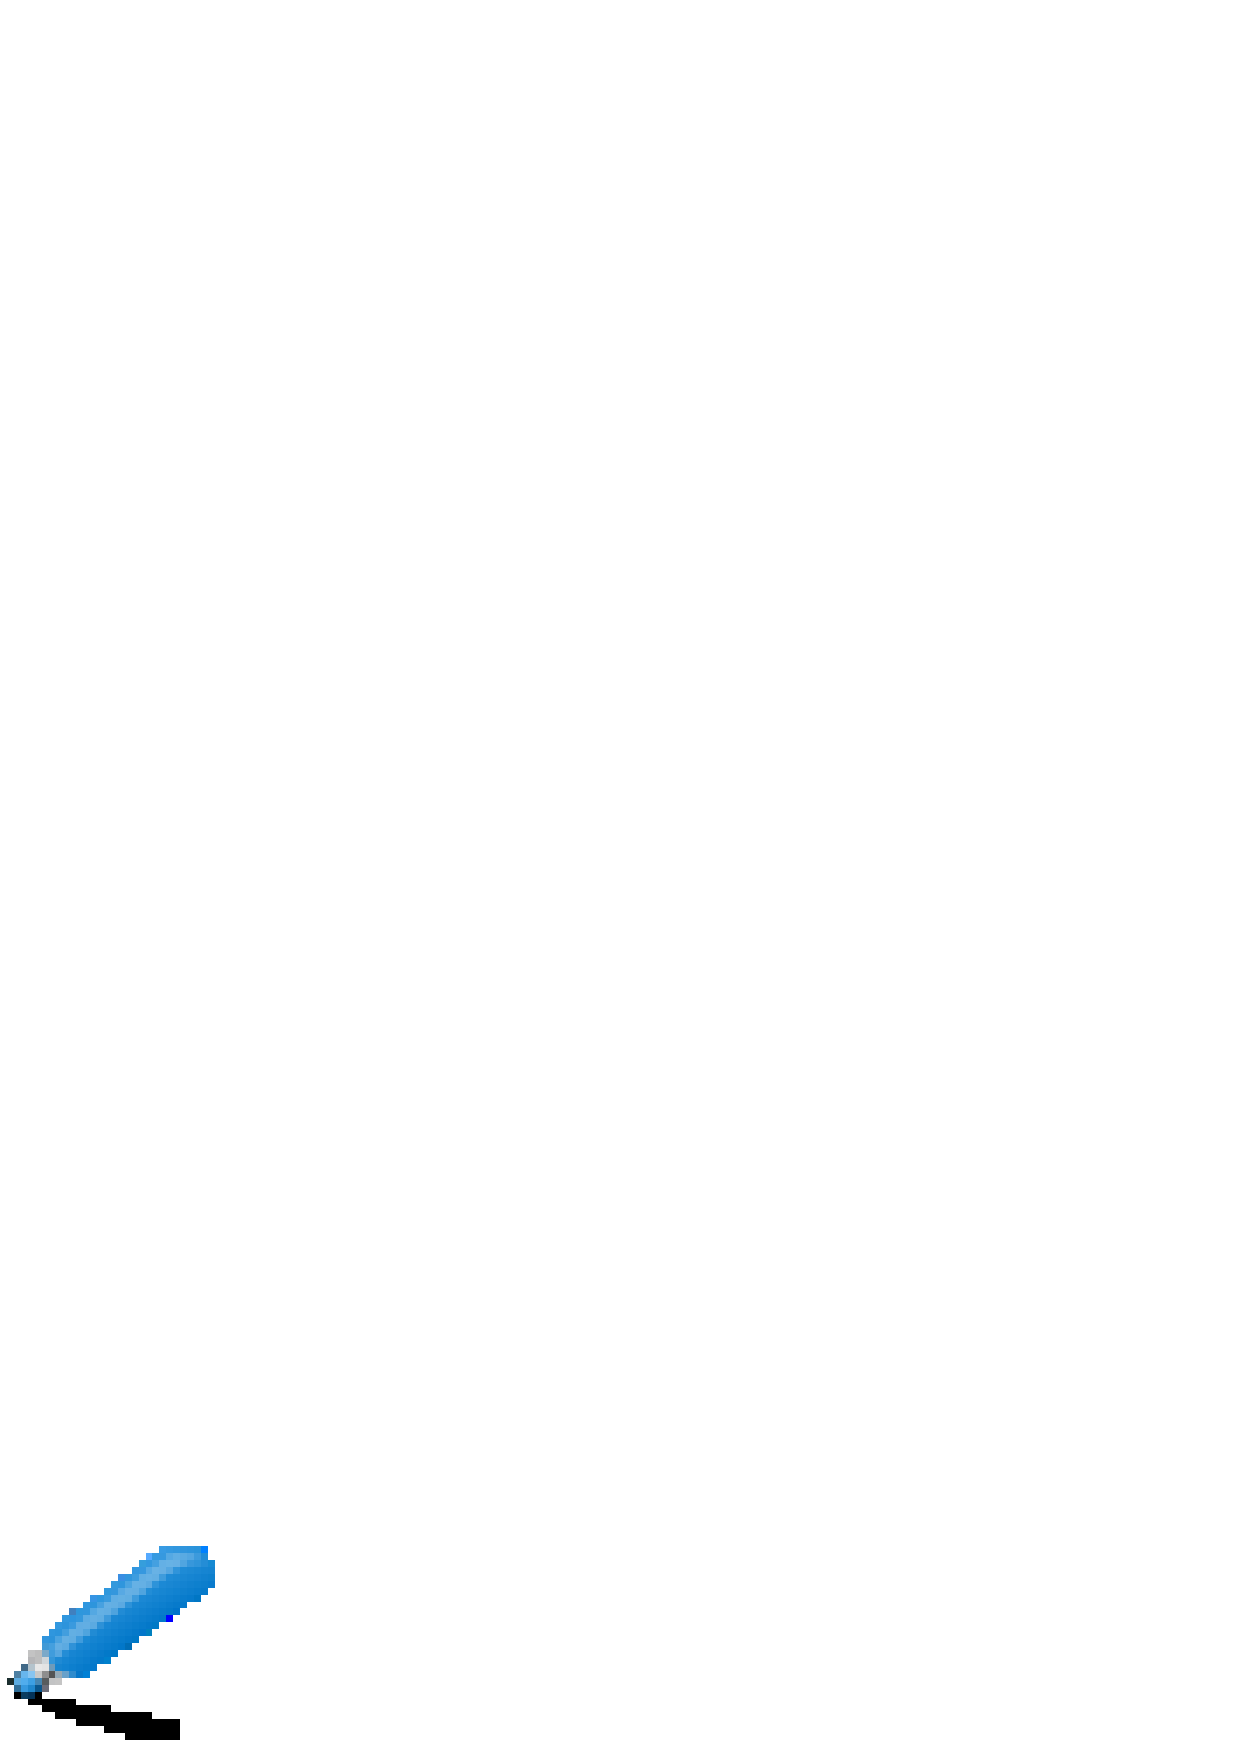
\includegraphics[width=0.5cm,clip=true]{mActionToggleEditing} ''Coordonnées de la position'' et cliquer sur \button{Nouvelle entité}. De la même façon, lorsque vous souhaitez enregistrer manuellement des sommets sans avoir activé ''Ajout automatique de sommets"  vous devez cliquer sur \button{Nouveau sommet} dans ce même écran.

\FloatBarrier
